% Intended LaTeX compiler: xelatex
\documentclass[a4paper, 12pt]{article}
\usepackage{graphicx}
\usepackage{grffile}
\usepackage{longtable}
\usepackage{wrapfig}
\usepackage{rotating}
\usepackage[normalem]{ulem}
\usepackage{amsmath}
\usepackage{textcomp}
\usepackage{amssymb}
\usepackage{capt-of}
\usepackage{hyperref}
\usepackage[danish]{babel}
\usepackage{mathtools}
\usepackage[margin=3.0cm]{geometry}
\hypersetup{colorlinks, linkcolor=black, urlcolor=blue}
\setlength{\parindent}{0em}
\parskip 1.5ex
\author{Matematik A}
\date{Vibenshus Gymnasium}
\title{Vektorfunktioner\\\medskip
\large Rette linjer og cirkler}
\hypersetup{
 pdfauthor={Matematik A},
 pdftitle={Vektorfunktioner},
 pdfkeywords={},
 pdfsubject={},
 pdfcreator={Emacs 27.2 (Org mode 9.4.4)}, 
 pdflang={Danish}}
\begin{document}

\maketitle
I dette skriv skal vi arbejde med rette linjer og cirkler som vektorfunktioner.

Først vil I blive introduceret til den rette linje som vektorfunktion. Derefter skal I regne to simple opgaver om netop dette. Dernæst vil I blive introduceret til en jævn cirkelbevægelse beskrevet som en vektorfunktion, hvorefter I igen skal regne to simple opgaver.

Efter opgaveregningen skal vi arbejde med "animationer" af vektorfunktioner i geogebra. Jeg demonstrerer i første omgang og siden prøver I selv.

Til sidst skal I arbejde med bestemmelse af hastigheds- og accelerationsvektorerne for en jævn cirkelbevægelse ved hjælp af differentialregning. Dette kommer til at foregå i jeres makkerpar og mundtligt.

\section*{Den rette linje som vektorfunktion}
\label{sec:org164bd8f}
\begin{figure}[htbp]
\centering
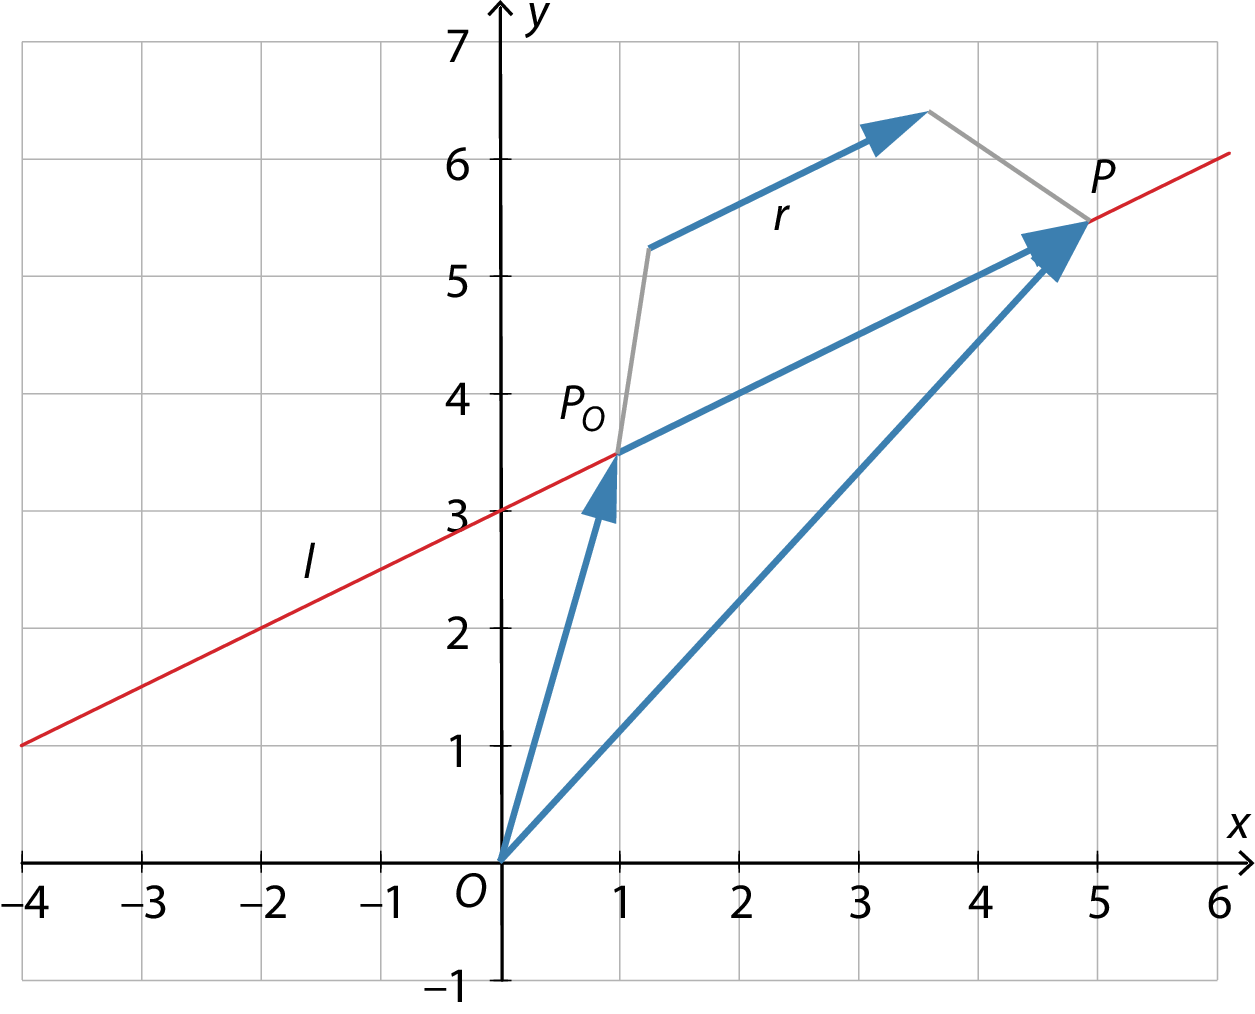
\includegraphics[width=0.5\linewidth]{img/ret_linje.png}
\caption{En ret linje som vektorfunktion.}
\end{figure}

En ret linje gennem et fast punkt \(P_0 = (x_0, y_0)\) og med retningsvektoren:

$$\vec{r}(t) = \begin{pmatrix} r_x \\ r_y \end{pmatrix}$$

har parameterfremstillingen(vektorfunktionen):

$$\overrightarrow{OP}(t) = \begin{pmatrix} x(t) \\ y(t) \end{pmatrix} = \begin{pmatrix} r_x \cdot t + x_0 \\ r_y \cdot t + y_0 \end{pmatrix}\..$$

\section*{Simple regneopgaver om rette linjer}
\label{sec:orgad12cd7}

Husk at vise formlen, som skal bruges. Skriv forklarende tekst. Medtag mellemregninger.

\subsection*{Opgave 1}
\label{sec:org5de1516}

En ret linje \(L\) går gennem punkterne \(A=(4, -1)\) og \(B=(1, 2)\).

\begin{enumerate}
\item Opstil en vektorfunktion for \(L\).
\end{enumerate}

\subsection*{Opgave 2}
\label{sec:orgcbd92d2}

En ret linje med hældningstallet \(a=2.5\) skærer x-aksen i punktet \(P_x = (4, 0)\).

\begin{enumerate}
\item Opstil en parameterfremstilling for linjen.
\end{enumerate}


\subsection*{Opgave 3}
\label{sec:orge9c295e}
En ret linje er givet ved vektorfunktionen:

$$\vec{r}(t) = \begin{pmatrix} t -1 \\ 3 + 2\cdot t \end{pmatrix}$$

\begin{enumerate}
\item Beregn linjens skæring med y-aksen.
\item Beregn linjens skæring med x-aksen.
\item Undersøg om punktet \(P=(-3,7)\) er beliggende på \(\vec{r}(t)\).
\item Omskriv vektorfunktionen til en almindelig funktion af typen \(f(x) = a \cdot x + b\).
\end{enumerate}

\newpage

\section*{Introduktion til cirklen}
\label{sec:org52e674b}

\begin{figure}[htbp]
\centering
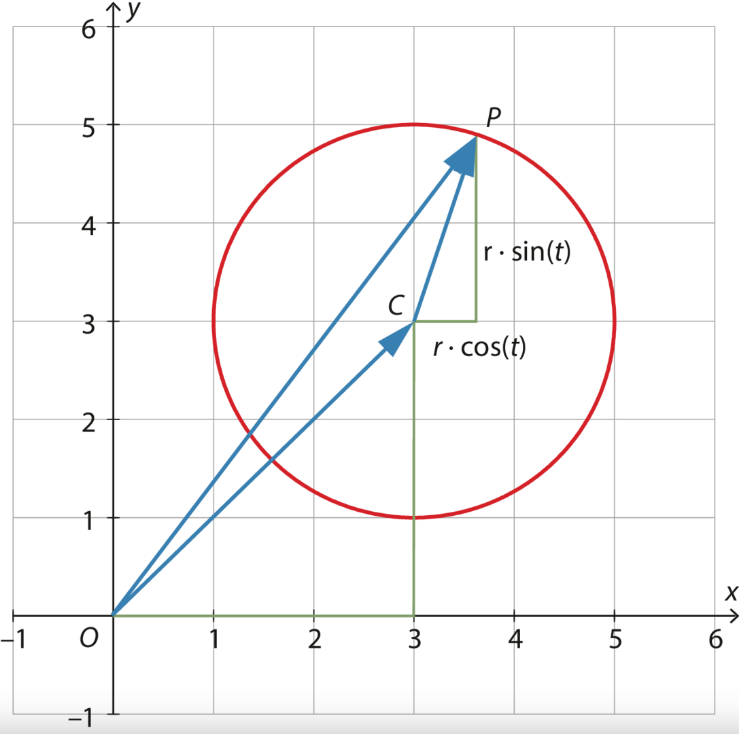
\includegraphics[width=0.5\linewidth]{img/2021-08-05_16-20-30_screenshot.png}
\caption{En cirkel som en vektorfunktion. Figuren er lånt fra jeres ibog \url{https://mathtxa.systime.dk}. Læg mærke til at vinkelhastighed og faseforskydning ikke er medtaget.}
\end{figure}


Et objekt som udfører en jævn cirkelbevægelse kan beskrives med følgende generelle parameterfremstilling:

$$\overrightarrow{OP}(t) = \begin{pmatrix} x(t) \\ y(t) \end{pmatrix} = \begin{pmatrix} x_0 \\ y_0 \end{pmatrix} + \begin{pmatrix} r \cdot \cos \left( \omega \cdot t + \phi \right) \\ r \cdot \sin \left(\omega \cdot t + \phi \right) \end{pmatrix} \.,$$

hvor \(P_0 = (x_0, y_0)\) er centrumskoordinatet til cirklen, \(r\) er radius i cirklen, \(\omega\) er vinkelhastigheden og \(\phi\) er faseforskydningen.

\newpage

\section*{Simple regneopgaver om cirkler}
\label{sec:org9f2c61c}

Husk at vise formlen, som skal bruges. Skriv forklarende tekst. Medtag mellemregninger.

\subsection*{Opgave 4}
\label{sec:org05b0d73}

Et objekt bevæger sig rundt på periferien af en cirkel givet ved ligningen:

$$(x-4)^2 + (y+2)^2 = 25\,.$$

med en vinkelhastighed på 3 s\textsuperscript{-1} og en faseforskydning på \(- \frac{\pi}{2}\).

\begin{enumerate}
\item Omskriv ligningen til en vektorfunktion.
\item Afbild vektorfunktionen i et koordinatsystem.
\end{enumerate}

\subsection*{Opgave 5}
\label{sec:org6a86260}

En cirkelbue er beskrevet ved vektorfunktionen:

$$\vec{r} (t) = \begin{pmatrix} 1 - \cos(t) \\ 3 + \sin(t) \end{pmatrix} \, , \, \text{hvor } 1 \leq t \leq 2 \,.$$

\begin{enumerate}
\item Beregn buens radius.
\item Beregn koordinaterne til buens centrum.
\item Beregn koordinaterne til buens endepunkter.
\item Beregn koordinaterne til det punkt, hvor \(t=1.8\).
\end{enumerate}

Et punkt på buen har koordinaterne \((x,y) = (0.733,y)\).

\begin{enumerate}
\setcounter{enumi}{4}
\item Beregn punktets tilhørende \(t\)​-værdi.
\item Afbild alle oplysninger om cirkelbuen og punktet i et koordinatsystem.
\end{enumerate}

\section*{Animation i geogebra af vektorfunktioner}
\label{sec:org39375d8}

Jeg viser jer, hvordan banekurver og stedvektorer kan tegnes og animeres i geogebra. Efterfølgende er det jeres opgave, at animere jeres løsninger til opgaverne.

\section*{Udledning af hastigheds- og accelerationsvektorer for den jævne cirkelbevægelse vha. differentiation på tavlen i makkerpar}
\label{sec:orgdbb19cb}

Her i den sidste øvelse skal I finde sammen i jeres makkerpar. Øvelsen går ud på mundtlig formidling til jeres makkere, ligesom da I skulle gennemgå beviser for hinanden. I skal arbejde med den jævne cirkelbevægelse beskrevet med vektorfunktionen:

$$\overrightarrow{OP}(t) = \begin{pmatrix} x(t) \\ y(t) \end{pmatrix} = \begin{pmatrix} x_0 \\ y_0 \end{pmatrix} + \begin{pmatrix} r \cdot \cos \left( \omega \cdot t + \phi \right) \\ r \cdot \sin \left(\omega \cdot t + \phi \right) \end{pmatrix} \..$$

\begin{description}
\item[{Makker 1}] Bestem et udtryk for hastighedsvektorfunktionen ved at differentiere stedvektorfunktionen. Undersøg den indbyrdes orientering af henholdsvis stedvektorfunktionen og hastighedsvektorfunktionen gennem brug at det, som hedder tværvektorer.

\item[{Makker 2}] Bestem et udtryk for accelerationsvektorfunktionen ved at differentiere hastighedsvektorfunktionen, som makker 1 lige har udledt. Undersøg den indbyrdes orientering af stedvektorfunktionen og nu accelerationsvektorfunktionen. Overvej, hvad modsatte vektorer er.
\end{description}
\end{document}